\documentclass[11pt]{article}

\usepackage{graphicx}
\usepackage{hyperref}
\usepackage{natbib}
\usepackage{amsmath}

\bibliographystyle{plain}  % or unsrt, alpha, etc.
\setlength{\textwidth}{6.5in}
\setlength{\headheight}{0in}
\setlength{\textheight}{8.0in}
\setlength{\hoffset}{0in}
\setlength{\voffset}{0in}
\setlength{\oddsidemargin}{0in}
\setlength{\evensidemargin}{0in}


\title{Computational Physics -  Problem Set 4}
  
\author{Frederik Holst Knudsen}


\begin{document}

\maketitle
Github URL: https://github.com/frederikholst/phys-ga2000
\section{Newman 5.9}
The heat capacity of a sample of 1000 $cm^3$ solid aluminum with $\rho =6.022 \times 10^{28}m^3$ and a debye temperature of $\theta_D = 428K$ is found using Gaussian quadrature integration. The weights and roots are found using numpy methods. The limits are accordingly scaled and the heat capacity is found to be 289 J/K.

The heat capacity from T=5K to T=500K is shown in Figure \ref{T-series}

\begin{figure}[!htbp]
    \centering
    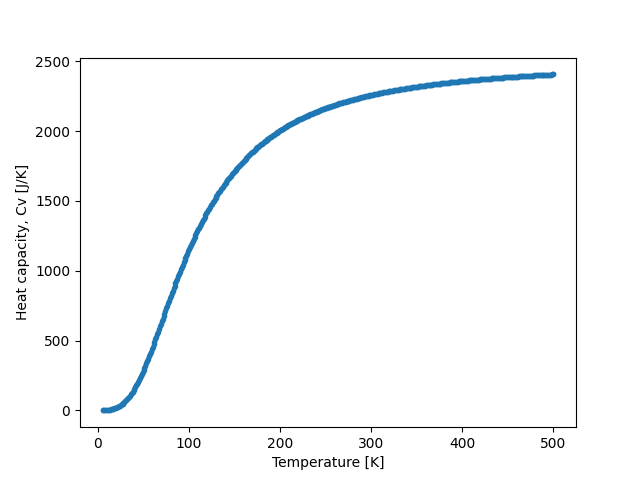
\includegraphics[width=0.7\textwidth]{T_series.png}
    \caption{The heat capacity is plotted against temperature for a sample of aluminum.}
    \label{T-series}
\end{figure}

Finally, Figure \ref{Conv} shows how the integration converges as we increase the sample points, where we see robust results already after a very few number of sample points. 

\begin{figure}[!htbp]
    \centering
    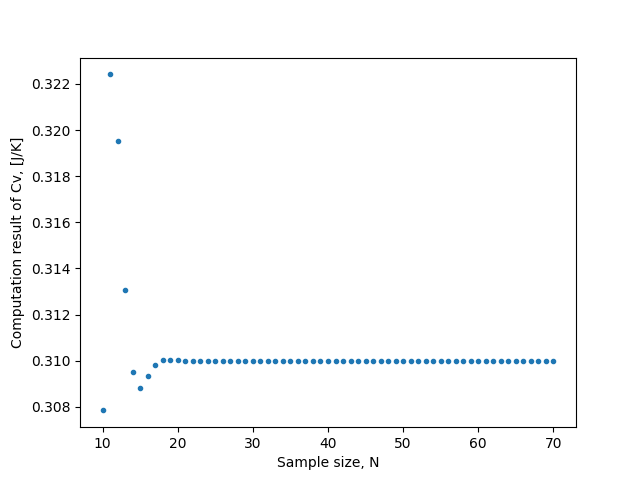
\includegraphics[width=0.7\textwidth]{Convergence.png}
    \caption{The computation of the heat capacity is plotted against sample points for the Guassian quadrature integration method. We see convergence already at around N=20 for T=5K. }
    \label{Conv}
\end{figure}

\section{Newman 5.10}
We derive the period of an anharmonic oscillator, where $E=V(a)$:

$$E=\frac{1}{2}m (\frac{dx}{dt})^2+V(x)$$

$$\sqrt{\frac{2}{m}(V(a)-V(x))}=\frac{dx}{dt}$$

$$dt=\sqrt{\frac{m}{2}}\frac{dx}{\sqrt{V(a)-V(x)}}$$

$$\int_{0}^{\frac{T}{4}}dt=\sqrt{\frac{m}{2}}\int_{0}^{a}\frac{dx}{\sqrt{V(a)-V(x)}}$$
$$T=\sqrt{8m}\int_{0}^{a}\frac{dx}{\sqrt{V(a)-V(x)}}$$

We now set $V(x)=x^4$ and $m=1$ and compute the period, T using Gaussian Quadratures with 20 sample points from $a=0$ to $a=2$ as seen in Figure \ref{Period}.

\begin{figure}[!htbp]
    \centering
    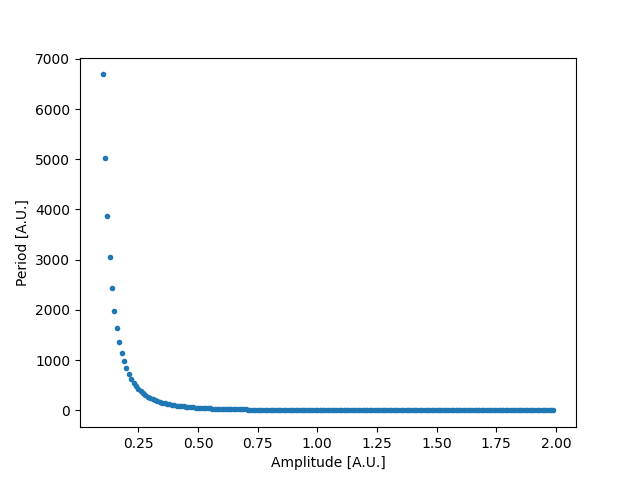
\includegraphics[width=0.7\textwidth]{Periods.png}
    \caption{The period, T is computed against amplitude, a. The point a=0 is excluded to avoid dividing with zero.}
    \label{Period}
\end{figure}

We find that the oscillator swings faster and faster the larger the amplitude. This is the case for the potential, $V(x)=x^4$, because any amplitude larger than the order of unity will amplify the restoring force by a large amount. Conversely, amplitudes smaller than unity will leave the restoring force equal to zero up to third order and reduced so much with the (almost) flattened potential of $x^4$. In the limit of $a$ going to zero, the motion will stop altogether, with the period going to infinity.  

\section{Newman 5.13}
Part A: We implement a recursive function that computes the Hermite polynomials and plot the wavefunctions of the harmonic oscillator of the order n=0,1,2,3 as seen in Figure \ref{x4}.

\begin{figure}[!htbp]
    \centering
    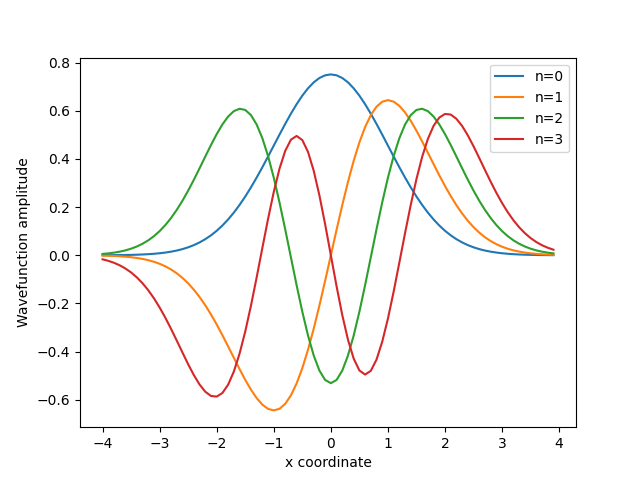
\includegraphics[width=0.7\textwidth]{Wavefunctions_n1-3.png}
    \caption{The four first wavefunctions of order n=0,1,2,3, are plotted in the range x=-4,x=4.}
    \label{x4}
\end{figure}

Part B: In figure \ref{partb} we see the wavefunction of order n=30:
\begin{figure}[!htbp]
    \centering
    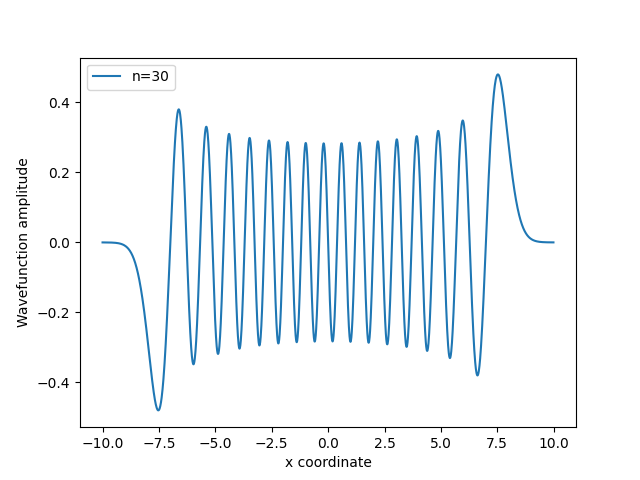
\includegraphics[width=0.7\textwidth]{Wavefunctions_n30.png}
    \caption{The wavefunctions of order n=30, is plotted in the range x=-10,x=10.}
    \label{partb}
\end{figure}

Part C: Using first Gaussian quadrature, we compute the uncertainty of the wavefunction with 100 sample points for n=5 and achieve the result: $\sqrt{\langle x^2\rangle }=2.3452078799117193$. 

Part D: Finally using Gauss-Hermite quadrature, we use scipy to give the roots and weights for 9 sample points and evaluate the integral to be $\sqrt{\langle x^2\rangle}= 2.3452078799117224$. Compared to the theoretical value of $\sqrt{\frac{11}{2}} $ this gives an error of -8.43769498715119e-15. So unfortunately not exactly zero approximation error but impressively close, considering only 9 sample points.

\end{document}



